\subsection{Distributed File Sharing}
\label{subsec:design-p2p}

\subsubsection*{Hash Tree}
\label{subsubsec:hash-tree}

The hash tree of a given directory is a tree object that stores information about its structure and contents. This is used to tell users what information they need to download, where it goes and what its contents should be. For every file, the hash tree stores a series of SHA-256 hashes. 

\begin{figure}[ht]
  \centering
  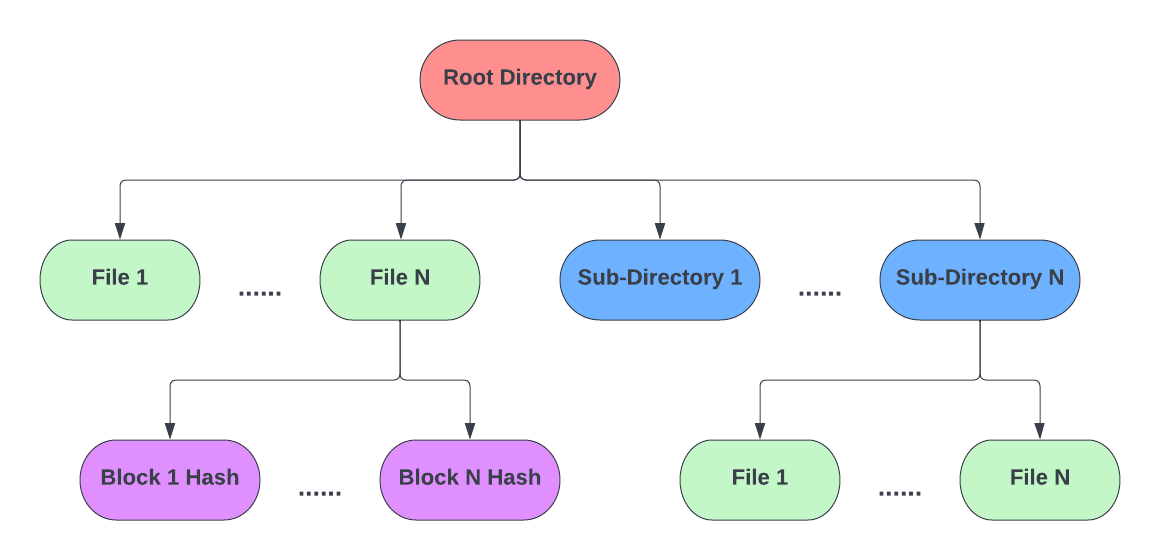
\includegraphics[width=.85\textwidth]{assets/images/diagrams/block-body.png}
  \caption{The structure of a hash tree}
  \label{fig:hash-storage}
\end{figure}

\subsubsection*{Uploading Content}
\label{subsubsec:upload-content}

For a developer to upload their game \reqref{F-M5} they must provide the required metadata outlined in Section~\ref{subsubsec:eth-data} as well as the location of the game in storage. A hash tree is then produced of the game and this is uploaded to IPFS, and the metadata about the game is uploaded to Ethereum.

\subsubsection*{Downloading Content}

Like mentioned in Section~\ref{subsec:design-data}, it is impractical to store the game's data on the blockchain or even IPFS. Instead we will consider ideas from decentralised file-sharing networks, like BitTorrent, to facilitate the distribution of content.
\x
Games are content addressable and are identified by their root hashes, which are stored on the blockchain and are calculated from the hash tree. Users will send messages using this hash to identify other users who are also interested in the same content \reqref{F-M3}, so they can share data. When two nodes connect to share content the node seeking content will:

\begin{enumerate}
  \item send their ethereum address along with an encrypted message to prove their address. The address is then looked up on the purchase list stored in the game's entry on the blockchain \reqref{F-S2}.
  \item Request individual shards from the node using the shard's hash \reqref{F-M2}.
  \item Use the hash tree, which has been fetched from IFPS, to verify the shard's contents \reqref{F-M7}.
  \item Send an encrypted encrypted certificate that the sender can use to prove their contribution.
  \item Repeat this for an arbitrary number of shards.
\end{enumerate}

\subsubsection*{Updating Content}

To satisfy \reqref{F-M4}, developers will perform the same steps outlined in Section~\ref{subsubsec:upload-content} but must also provide the root hash of the most previous version of the game. Any users who have purchased the previous version, will be added to the list of users who have purchased the new version. Additionally, this will include the restriction that only the original uploader can upload an update for their game \reqref{NF-S2}.
\x
Each version is considered as its own game and will require users to download the updated version separately. Whilst this isn't reflective of how updates are typically managed, this will be acceptable for the scope of this project and any changes will be considered as a future extension to this project.

\subsubsection*{Downloadable Content}
% TODO
\tbd

% {F\_S3}) for their games that users will purchase separately. Each DLC will need:

% \begin{enumerate}
%   \item \textbf{Dependency} A reference to the oldest version of the game they apply to, and
%   \item \textbf{Previous Version} A pointer to the previous version of the DLC.
% \end{enumerate}

% \begin{figure}[ht]
%   \centering
%   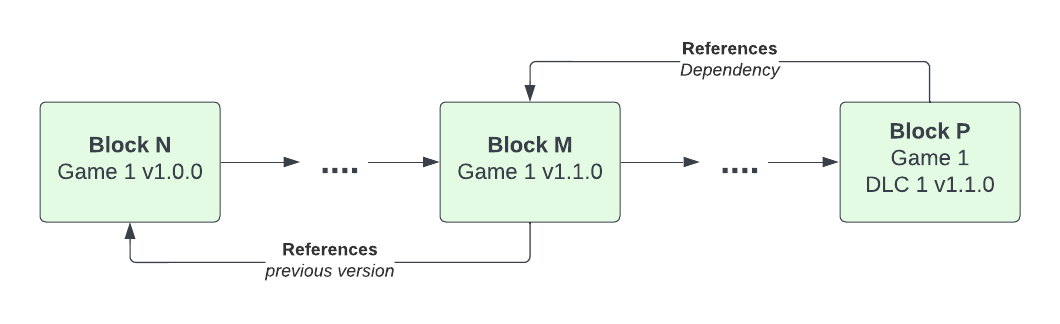
\includegraphics[width=.85\textwidth]{assets/images/diagrams/software.png}
%   \caption{How blocks relate to each other. An update will reference the previous version whilst a DLC will reference, which piece of software and version it is dependent on.}
% \end{figure}

\subsubsection*{Proving Contribution}

When a user successfully downloads a shard of data, they will reply with a confirmation certificate to prove that they have downloaded the game. Each Ethereum address is related to a public/private key pair so a confirmation certificate will be encrypted by a given node's private key to prove authenticity. A user will prove their contribution \reqref{F-S1} by sending a collection of certificates to the uploader, who will validate them and reward the user accordingly.